
\chapter{相关技术综述}

\section{消息队列 RocketMQ}

Apache RocketMQ 是一种高性能、高可靠的分布式消息中间件，最初由阿里巴巴提出并开源，现已成为 Apache 顶级项目，广泛应用于异步通信、系统解耦和流量控制等业务场景。RocketMQ 采用发布—订阅（Publish-Subscribe）的消息模型，支持点对点和广播等多种消费方式，能够满足大规模分布式系统中对消息传递可靠性和稳定性的要求。

在消息组织方式上，RocketMQ 以主题（Topic）作为消息管理的基本单位，消息在 Broker 中按照队列（Queue）进行存储和分发。通过将同一主题下的消息分布到多个队列中，系统可以实现消息的并行写入和并行消费，从而提升整体吞吐能力。在消息存储方面，RocketMQ 采用顺序写磁盘的方式进行消息持久化，在保证可靠性的同时提高了写入效率。

在消息投递与消费机制方面，RocketMQ 支持生产者向指定主题发送消息，由消费者以订阅方式进行消费，并通过消费进度管理和投递确认机制保障消息的可达性。系统支持至少一次（At-Least-Once）的消息投递语义，并提供顺序消息和延迟消息等能力，使其能够适应对消息时序性和定时触发有要求的业务场景。

在系统架构层面，如图\ref{fig:rocketmq_architecture}所示，RocketMQ 由 NameServer、Broker、Producer 和 Consumer 等组件构成。NameServer 负责维护集群的路由信息，Broker 负责消息的存储与转发，Producer 和 Consumer 分别承担消息的生产与消费职责。该架构采用去中心化设计，支持 Broker 节点的动态扩展和故障转移，在节点异常情况下能够保证消息服务的连续性。

在分布式系统中，RocketMQ 常用于构建基于事件驱动的消息通信机制，通过消息队列对请求进行缓冲和调度，降低系统之间的直接依赖关系。同时，消息队列能够在高并发场景下对突发流量进行削峰填谷，并通过消费速率控制实现限速处理，从而提升整体系统的稳定性和可扩展性。

\begin{figure}[!htbp]
  \centering
  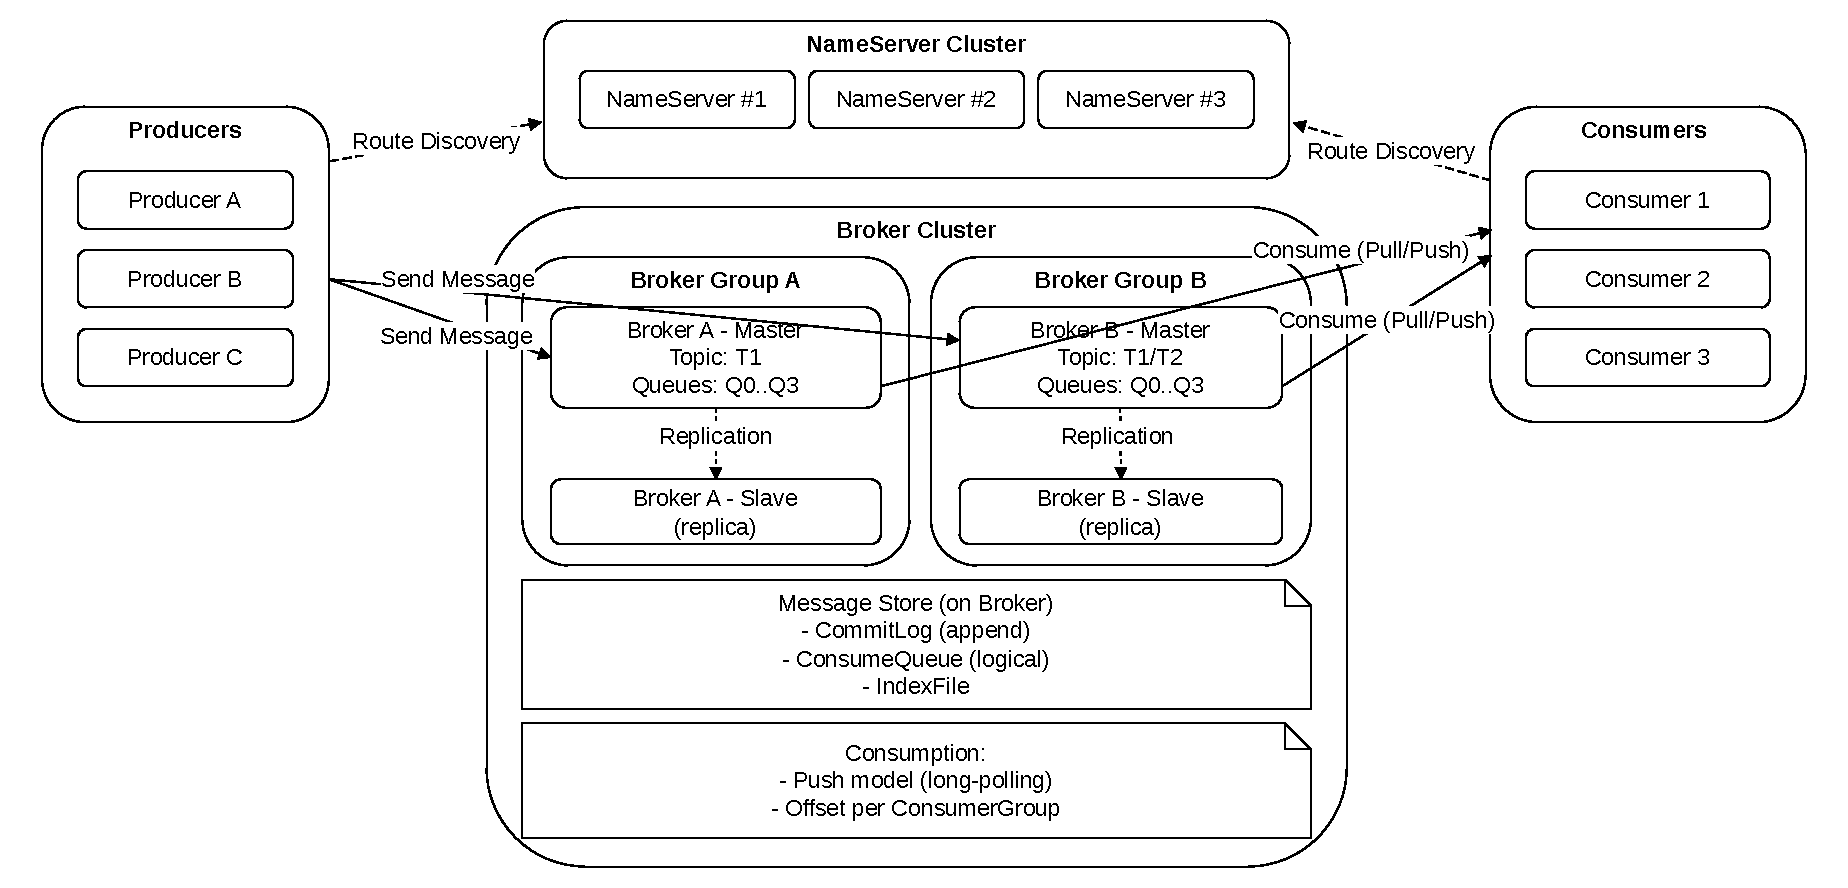
\includegraphics[width=1.0\linewidth]{./figure/figures-RocketMQ架构图.drawio.pdf}
  \caption{RocketMQ 架构图}
  \label{fig:rocketmq_architecture}
\end{figure}


\section{全文搜索引擎 Elasticsearch}

Elasticsearch 是一种基于 Lucene 的分布式搜索与分析引擎，面向文档（document）与字段（field）的数据模型，支持结构化、半结构化与非结构化内容的统一检索与聚合分析\cite{bialecki2012apache}。其核心目标是在横向扩展的集群上，以近实时（near real-time）的方式提供高并发、低延迟的检索能力。

从体系结构上，集群由多个节点（node）构成，索引（index）是逻辑管理单元，索引被划分为若干主分片与副本分片（shard），分布在不同节点上以实现水平扩展与容错。写入采用分段（segment）追加与后台合并策略，结合刷新（refresh）机制实现近实时可见性；分布式检索采用“scatter–gather”模式在多分片间并发执行、汇总与重排结果。

在 Lucene 内核层面，文档写入后会形成多个不可变段（segment），段内包含倒排索引、存储字段（stored fields）、词典与统计信息等。段不可变的设计使得读取路径可以高度优化，而更新与删除则以追加与标记方式实现，并在后台通过段合并（merge）逐步回收删除标记与优化索引结构。近实时特性来自“写入缓冲区 $\rightarrow$ 刷新生成新段 $\rightarrow$ 搜索器可见”的流程：刷新并非强制落盘（flush），而是将内存中的索引结构转换为可检索的段，从而在吞吐与时效之间取得折中。

在文本索引方面，如图\ref{fig:es_inverted_index}所示，文档字段首先经过分析器（analyzer）管线处理：字符过滤（character filter）统一规范化，分词器（tokenizer）切分词项，随后进行大小写、停用词、词干化或同义词等令牌过滤（token filter）。最终构建“词项 $\rightarrow$ 倒排列表 $\rightarrow$ 位置信息”的倒排索引结构，以支持关键词匹配、短语匹配与邻近度查询。

\begin{figure}[!htbp]
  \centering
  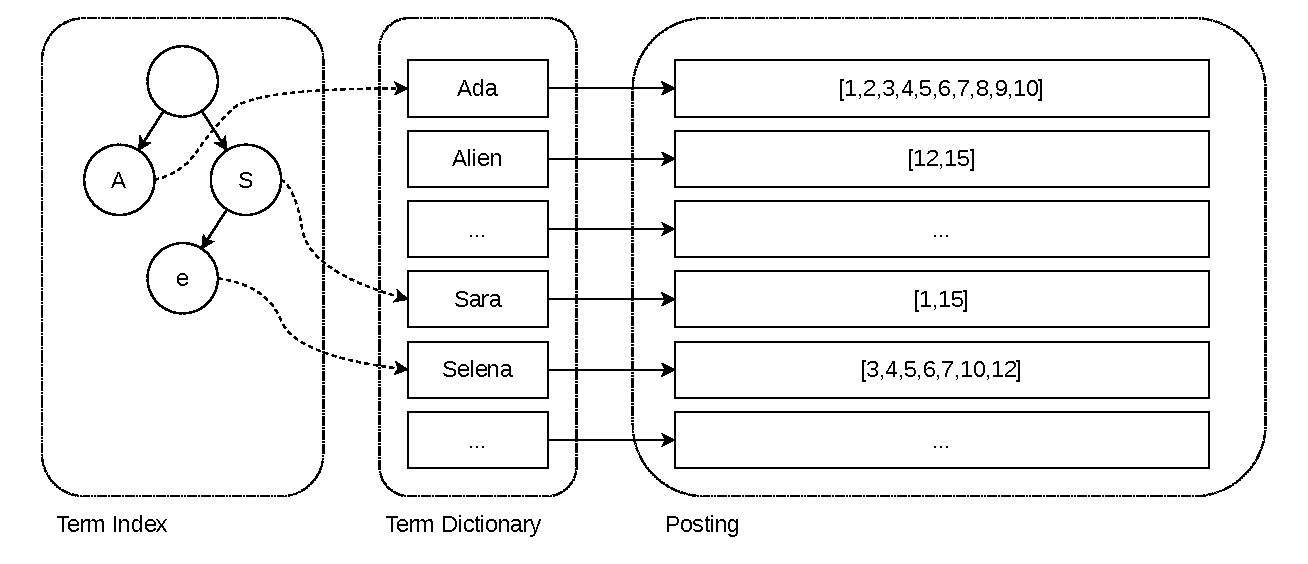
\includegraphics[width=1.0\linewidth]{./figure/figures-ES倒排索引.drawio.pdf}
  \caption{Elasticsearch 倒排索引示意图}
  \label{fig:es_inverted_index}
\end{figure}

在相关性计算方面，系统采用基于概率相关性的 BM25 打分，对词频、逆文档频率与字段长度进行归一化建模，兼顾高频项的收益递减与长文惩罚\cite{bialecki2012apache}。查询表达使用 DSL 组合布尔、短语、范围、多字段匹配等算子，结果可基于高亮、分页与聚合（aggregation）进行呈现。除倒排索引外，列式存储的 DocValues 支持高效的排序、去重与聚合统计。

在查询执行上，分布式检索通常包含两个阶段：查询阶段（query phase）在每个相关分片上计算候选集合与局部 TopK，随后在协调节点汇总并执行全局合并；当需要返回文档详情、字段或高亮时，还会触发取回阶段（fetch phase）从对应分片读取 stored fields 或 \_source。为降低跨分片开销，系统常在局部阶段尽量裁剪候选集合，并在全局阶段完成最终重排与分页。

聚合分析（aggregation）是 Elasticsearch 区别于传统检索系统的重要能力之一。通过 terms、histogram、range 等桶聚合（bucket aggregation）与 sum、avg、percentiles 等指标聚合（metric aggregation），系统能够在一次查询中同时完成“检索 + 统计”。其底层依赖 DocValues 的列式结构按字段扫描与分桶聚合，支持在大规模文档集合上进行近实时分析。

综上，Elasticsearch 通过“分布式分片—近实时索引—倒排结构—BM25 打分—聚合分析”的组合，实现了对大规模文档集合的高效关键词检索；其在内容检索、日志分析与监测告警等领域被广泛采用，并与稠密向量检索形成互补\cite{wang2021bert}。

\section{Embedding与Milvus}

Embedding 是将文本、图像等非结构化对象映射为稠密向量的一类表示学习方法，目标是在向量空间中保留语义相似性——语义相近的对象在空间中的距离更近。与基于关键词的稀疏表示相比，稠密向量能更好地涵盖同义改写与语义扩展，因此适用于语义召回与聚类等任务。

在表征层面，文本向量通常由预训练语言模型通过池化（如 CLS/平均池化）得到；相似度度量多采用余弦相似或内积。根据训练目标的不同，向量可以强调语义等价、主题相似或任务相关性，例如对比学习目标常用于增强“语义接近”的可分性。与词项级稀疏表示相比，稠密向量通过在连续空间中编码上下文信息，使得语义相近但词面差异较大的表达更容易被检索到。

在向量检索问题中，给定查询向量，需要在海量向量集合中返回相似度最高的 TopK 近邻。精确最近邻（Exact NN）在高维空间的复杂度与存储开销较高，因此近似最近邻（Approximate NN，ANN）成为主流路径：ANN 通过牺牲部分精确性换取显著的加速，并通过参数化控制召回率与时延之间的权衡。

Milvus 是面向向量数据的数据库系统，围绕索引构建、相似度检索与元数据过滤提供系统支持\cite{wang2021milvus}。其典型索引包括：基于聚类中心的 IVF（Inverted File）系列，用粗量化缩小检索候选；基于邻接图的 HNSW（Hierarchical Navigable Small World），以多层小世界图实现高效近邻搜索；以及结合产品量化（Product Quantization，PQ）的压缩索引，在牺牲部分精度的前提下降低存储与计算成本。

IVF 索引通常先对向量空间进行聚类，将向量分配到若干倒排桶中；检索时先选择与查询最接近的一小部分桶，再在桶内做局部搜索，从而显著减少候选规模。HNSW 则通过构建分层图结构，使搜索从稀疏高层开始逐步逼近，再在密集低层细化，具有较好的时延与召回表现。PQ 将高维向量分块并对每块进行量化编码，以更低的码长近似原向量，进而降低存储占用并加速相似度计算，但可能带来一定精度损失。

在系统层面，Milvus 通过服务端组件协同完成向量写入、索引构建与 TopK 检索，并支持与标量维度（如时间、类别）组合的过滤查询。面向带结构化过滤条件的向量检索场景，过滤式近似最近邻搜索的系统设计与性能权衡也逐渐成为研究重点，这进一步说明向量数据库不仅要处理相似度计算，还需要协调过滤、索引与延迟之间的关系\cite{wang2021milvus,patel2024acorn}。

\section{检索增强生成 RAG}

检索增强生成（Retrieval-Augmented Generation，RAG）是一类将外部知识检索融入生成过程的模型化框架，其动机在于缓解大语言模型面对知识密集型任务时的幻觉与时效性不足问题\cite{lewis2020retrieval}。RAG 通过为生成模型提供与输入相关的证据文档，使生成不再仅依赖参数内隐知识，从而在开放域问答、企业知识问答与面向业务规则的辅助决策等场景中表现出较强的可控性。从基本机制看，RAG 将“参数化知识”与“非参数化知识”结合起来：前者由预训练语言模型内化在模型参数中，负责语言组织、推理模式与回答表达；后者则由检索系统从外部知识库中动态提供，负责补充事实、时效信息与领域细节。二者结合后，模型不再试图仅凭参数记忆回答所有问题，而是通过“先找证据，再据此生成”的方式完成回答，这也是 RAG 区别于纯生成式问答的核心所在\cite{lewis2020retrieval}。

典型流程包括：问题表示与检索、候选融合与重排、证据组织与条件生成。首先，系统需要将用户问题转换为适合检索的表达形式，这一过程既可能是基于关键词的直接检索，也可能涉及问题改写、查询扩展与多路召回；其次，系统从稀疏检索、稠密检索或混合检索通道中获得候选证据，并通过去重、融合与重排提升候选集合质量；最后，系统将问题与筛选后的证据共同送入生成模型，在约束上下文窗口的前提下输出回答文本，并可进一步附带引用、出处或跳转信息。在检索侧，RAG 并不局限于单一召回机制。稀疏检索擅长命中显式术语与精确表达，适用于制度名词、产品名与规则编号等场景；稠密检索则更适合处理同义改写、口语化表达与跨表述方式的语义匹配。实际系统中，二者往往并行使用，再通过重排模型或启发式策略进行融合，以在召回率、准确率与延迟之间取得平衡。这种“混合召回 + 重排”的结构也逐渐成为工程实践中的主流方案\cite{fan2024survey,huang2025survey}。在生成侧，证据组织方式直接影响回答质量。若证据片段过长，会挤占上下文窗口并引入无关噪声；若片段过短，则可能破坏语义完整性，导致模型无法形成足够的上下文理解。因此，知识切片粒度、相邻片段合并策略、证据排序方式以及输入模板设计，都会显著影响最终生成效果。除“问题 + 若干片段”的直接拼接方式外，也有研究关注先对证据做聚合、摘要或压缩，再进入生成阶段，以提高证据利用效率\cite{fan2024survey}。

在模型融合形态上，既有“检索器 + 生成器”的级联方式，也有在解码阶段融合多文档证据的方案（如 FiD\cite{izacard-grave-2021-leveraging}）。此外，将重排与生成任务统一以提升证据利用率也是当前的研究热点\cite{yu2024rankrag}。从系统范式看，RAG 的关键挑战在于“检索质量—证据组织—生成一致性”的深度耦合：检索噪声与片段粒度直接影响生成，而有限的上下文窗口又要求对证据进行高效筛选与压缩。若证据间存在冲突或时效不一，模型极易产生事实不一致的回答。因此，证据选择、长上下文建模与一致性评价已成为该领域的核心方向\cite{fan2024survey,huang2025survey}。

面向工程落地时，RAG 是一类复杂的系统协同问题，其效果依赖知识库构建、权限过滤、查询改写与召回融合等环节。在企业场景中，动态内容、多样形态与细粒度权限要求系统不仅要保证相关性，还需满足时效性与合规约束。因此，RAG 必须与内容管理及权限控制深度整合。总体而言，RAG 结合了检索与生成，形成了“检索—重排—生成”范式，其应用重点正向证据高效利用与推理能力演进\cite{fan2024survey,yu2024rankrag,huang2025survey}。对于本文研究的内容平台而言，RAG 既是实现智能问答的基础，也是连接内容管理与前台体验的关键桥梁。

\section{本章小结}

本章围绕平台最关键的技术基座展开综述：消息中间件 RocketMQ、关键词检索引擎 Elasticsearch、Embedding 与 Milvus，以及检索增强生成（RAG）。其中，Elasticsearch 提供关键词检索与聚合分析能力，支撑页面化展示与结构化过滤；Embedding 负责将非结构化内容映射为稠密向量，Milvus 则围绕向量索引构建、近似最近邻检索与标量过滤提供系统支撑，二者共同构成语义召回能力；RAG 将关键词检索与语义检索结果进一步组织并注入生成模型，结合证据引用提升回答的可解释性与可控性；RocketMQ 提供事件驱动的异步解耦能力，支撑索引构建与数据回收链路。以上技术共同构成了“生产—发布—应用—治理—评估”的核心支撑。
